\section{Communication patterns}\label{section:applied-methods:communication-shell-remote}

The next step was to implement some form of communication between the application shell and the micro-frontends. This section focuses on the communication strategy implemented through injection tokens between the application shell and the micro-frontends. To further explain the communication pattern, the integration of the layout will be used as an example of this pattern.

\bigskip

\noindent To allow parallel development and deployment of micro-frontends, it is necessary that their implementation is as independent as possible. Two micro-frontends should not communicate directly with each other, as it creates a tight coupling. Instead, it is better that one micro-frontend communicates indirectly to the other micro-frontends by publishing events to a central event bus, and the other micro-frontends are subscribed to the events. This pattern is known as publish/subscribe mechanism. Alternatively, the application shell orchestrates the communication of the micro-frontends. One micro-frontend emits an event, which the application shell intercepts. The application shell propagates the event to the target micro-frontend afterwards. This approach drastically reduces the coupling between micro-frontends. The micro-frontend does not need implementation details about the other micro-frontends, allowing for parallel development.

\bigskip

\noindent As explained in Section \ref{subsection:background:micro-frontend:communication-patterns} three distinct types of communication can be used between micro-frontends and the application shell. Angular provides an excellent feature for implementing unidirectional communication between micro-frontends, namely \ac{DI}. The application shell can provide services that the micro-frontends can inject. An Angular injection token was created to implement certain behavior if an application runs in standalone mode or is run through an application shell.

\noindent An injection token can be used to define a dependency that should be injectable into a class. The token can be of any value, but the injected type is usually not reified, which means that it is not available at runtime. \cite{misc:-:applied-methods:communication:angular-injection-token}


\bigskip

\noindent The following paragraph describes the usage of the injection token inside the contact application, however, the usage is the same for every micro-frontend inside the architecture. The definition and the usage of the token is shown in Listing \ref{code:applied-methods:communication-patterns:providing-native-configuration}. The core module within the contact application provides the value for the token indicating that the application is running in standalone mode when the token can be injected. The token is injected by the contact's feature module, which is the module exposed via Module Federation. The module injects the token to run additional logic, it is consumed by the application shell. The application shell does not need to provide the injection token because the logic is not executed if the token is not defined.

\ifshowListings
\begin{listing}[H]
  \begin{minted}{typescript}

const CONTACT_NATIVE_ENVIRONMENT = 
  new InjectionToken<boolean>('CONTACT_NATIVE_ENVIRONMENT');

@NgModule({
  imports: [ ... ],
  providers: [{ provide: CONTACT_NATIVE_ENVIRONMENT, useValue: true }]
})
class ContactCoreModule {}
  \end{minted}
  \caption{Provide the application with the \texttt{CONTACT\_NATIVE\_ENVIRONMENT} injection token.}\label{code:applied-methods:communication-patterns:providing-native-configuration}
\end{listing}
\fi

\noindent A requirement of the architecture is that the micro-frontends should be able to integrate their navigation nodes into the application shell. The structure of the requirement is shown in Figure \ref{fig:applied-methods:communication-patterns:comparison-between-host-and-contact-layout}. Upon loading the contact micro-frontend in the application shell, the navigation row for the contact should be created below the navigation of the application shell.

\ifshowImages
  \begin{figure}[H]
  \centering
  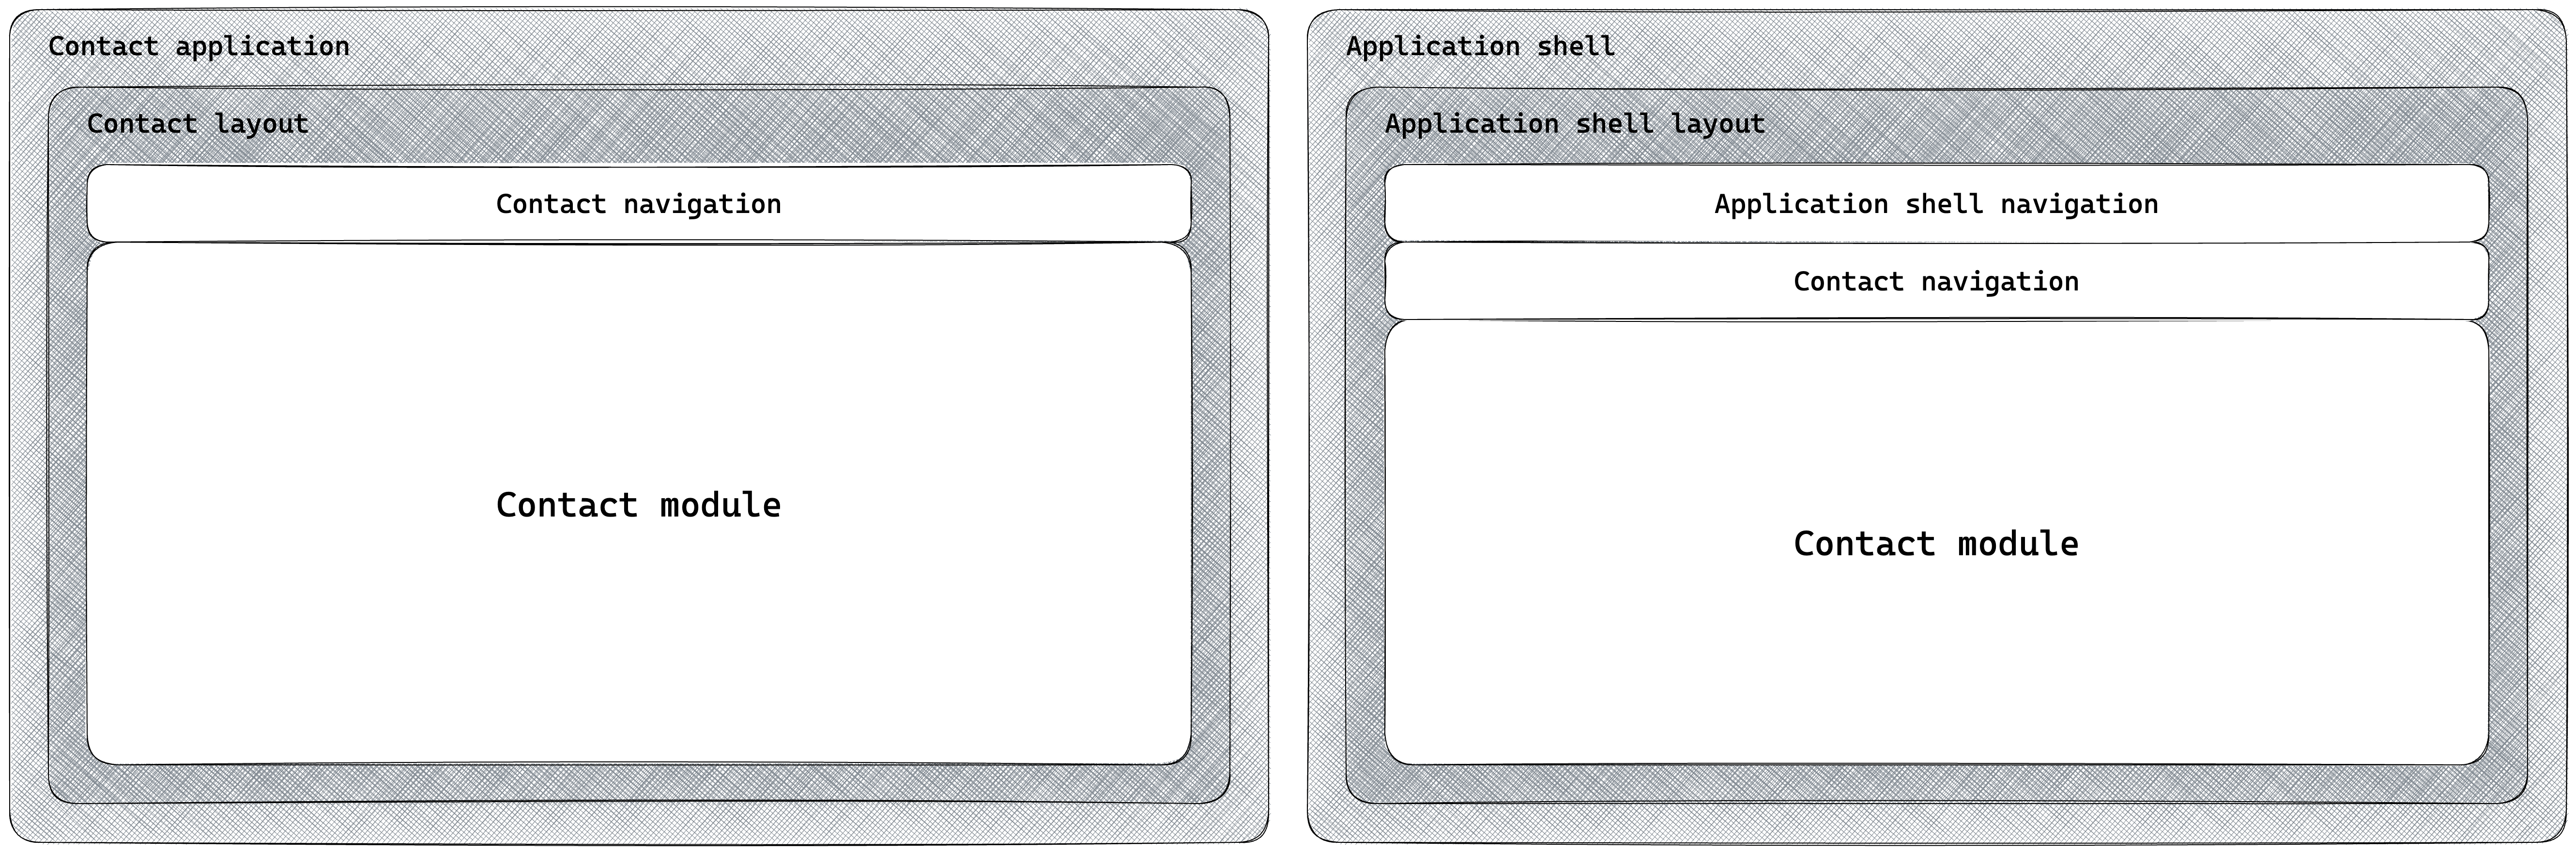
\includegraphics[width=1\linewidth]{images/applied-methods/communication-patterns/layout-comparison.png}
  \caption{A comparison between the navigation inside the contact application and the application shell.}\label{fig:applied-methods:communication-patterns:comparison-between-host-and-contact-layout}
  \end{figure}
\fi

\noindent Therefore, the application shell has to offer a mechanism to make it possible to integrate the micro-frontend navigation into the layout. To simplify the procedure, a layout service was created that can be injected by the micro-frontends. The layout service can register a second navigation row in the header. The logic for registering a second row inside the navigation is only executed if the micro-frontend is executed in the application shell. The difference between the navigation inside the application shell and the contact application can be seen in Figure \ref{fig:applied-methods:communication-patterns:contact-application-header} and \ref{fig:applied-methods:communication-patterns:application-shell-header}. The first figure shows the navigation row inside the contact micro-frontend. The second figure shows the navigation of the application shell, which incorporates the navigation of the contact micro-frontend in the second navigation row. The first row contains the navigation of the application shell, which links to the different micro-frontends. The second row is the navigation of the contact micro-frontend, which is only shown if the contact micro-frontend is currently active.

\ifshowImages
  \begin{figure}[H]
  \centering
  
\includegraphics[width=1\linewidth]{images/applied-methods/communication-patterns/contact-header.png}
  \caption{The navigation of the contact application.}\label{fig:applied-methods:communication-patterns:contact-application-header}
  \end{figure}
\fi

\ifshowImages
  \begin{figure}[H]
  \centering
  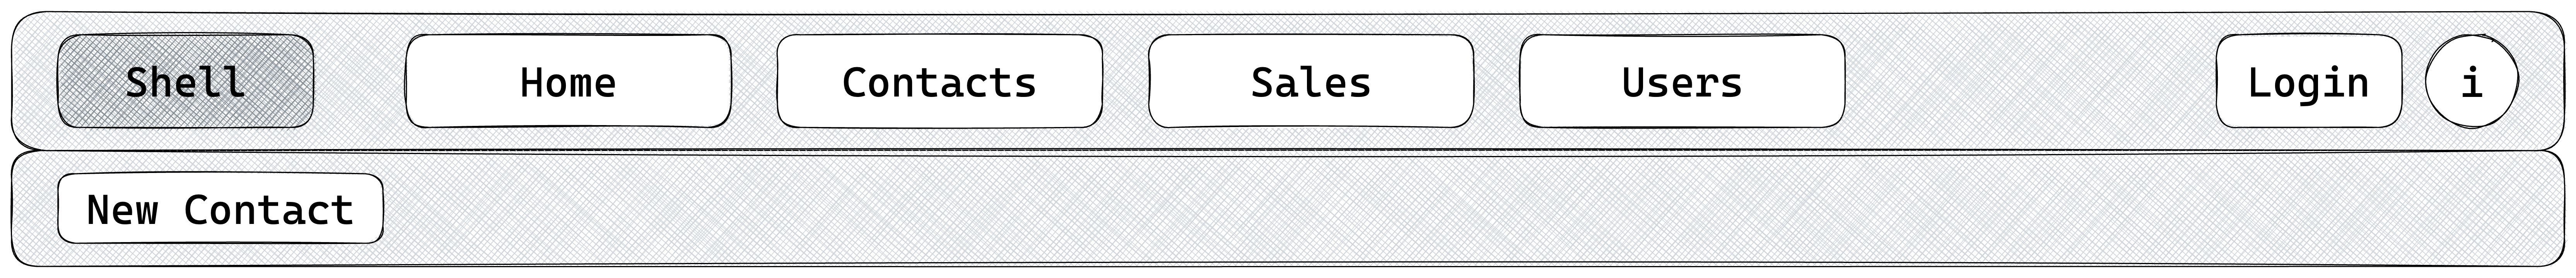
\includegraphics[width=1\linewidth]{images/applied-methods/communication-patterns/host-contact-header.png}
  \caption{The navigation of the application shell.}\label{fig:applied-methods:communication-patterns:application-shell-header}
  \end{figure}
\fi

\noindent Initialization logic has to be executed when a micro-frontend is rendered inside the application shell. This initialization logic registers the second navigation toolbar. Upon navigating to a micro-frontend, the second navigation row is registered, and it is removed upon navigating away from the micro-frontend. The initialization steps are only executed if the micro-frontend is running inside the application shell. A part of the workflow to register and remove the second toolbar row is shown in the Listing \ref{code:applied-methods:communication-patterns:initialization-logic-micro-frontend}.

\ifshowListings
\begin{listing}[H]
  \begin{minted}[escapeinside=||]{typescript}
|#|isNative = inject(CONTACT_NATIVE_ENVIRONMENT, { optional: true });
|#|layoutService = inject(LayoutService);

init(): void {
  if (!this.|#|isNative)
    const { topNodes } = CONTACT_NAVIGATION;
    this.|#|layoutService.registerSecondToolbarRow(topNodes);
}

ngOnDestroy(): void {
  if (!this.|#|isNative)
    this.|#|layoutService.unregisterSecondToolbarRow();
}
  \end{minted}
  \caption{An part of the initialization process of a micro-frontend.}\label{code:applied-methods:communication-patterns:initialization-logic-micro-frontend}
\end{listing}
\fi

\subsection{Layout integration}\label{subsection:applied-methods:communication-patterns:layout-integration}

At first, it was troublesome to integrate the remote module into the layout. Therefore the layout service was created with the \texttt{forRoot} and \texttt{forChild} pattern. This pattern typically provides different configuration options for a feature module.

\bigskip

\noindent Here's how it works:

\begin{itemize}
  \item The \texttt{forRoot} function is typically called in the application root module to provide configuration options for a global feature module to the entire application. This method usually returns a module with all providers available globally.
  \item The \texttt{forChild} function is called in a child module that imports the feature module to provide configuration options that are specific to that module. This method usually returns a module with providers only available to components and services within that child module.
\end{itemize}

\noindent The Listing \ref{code:applied-methods:communication-patterns:layout-module} shows the implementation of the \texttt{forRoot} and \texttt{forChild} pattern inside the layout-module.

\ifshowListings
  \begin{listing}[H]
  \begin{minted}{typescript}
class LayoutModule {
  static forRoot(): ModuleWithProviders<LayoutModule> {
    return {
      ngModule: LayoutModule,
      providers: [LayoutNavigationService, LayoutTemplateService],
    };
  }

  static forChild(): ModuleWithProviders<LayoutModule> {
    return { ngModule: LayoutModule };
  }
}
  \end{minted}
  \caption{The implementation of \texttt{forRoot} and \texttt{forChild} inside the layout module.}\label{code:applied-methods:communication-patterns:layout-module}
  \end{listing}
\fi

\noindent This approach allows the \texttt{LayoutNavigationService}- and \texttt{LayoutTemplateService}-services available in the root injector. These services can be used to register navigation nodes and templates inside the header. The \texttt{LayoutModule.forChild()} can be used where the components and directives of the layout are needed. Providing the \texttt{LayoutModule} in the root module is shown in the Listing \ref{code:applied-methods:communication-patterns:importing-the-root-layout-module}

\ifshowListings
  \begin{listing}[H]
  \begin{minted}{typescript}
@NgModule({
  imports: [ LayoutModule.forRoot() ],
})
class ContactCoreModule {}
  \end{minted}
  \caption{Provide the layout services to the root injector.}\label{code:applied-methods:communication-patterns:importing-the-root-layout-module}
  \end{listing}
\fi
